\documentclass[aspectratio=149]{beamer}

\usepackage[utf8]{inputenc}
\usepackage[T1]{fontenc}

\usepackage[english]{babel}
\usepackage{amsmath}
\usepackage{cleveref}
\usepackage{amssymb}
\usepackage{mathtools}

%%Numbers, expectation
\newcommand{\N}{\mathbb{N}}
\newcommand{\E}{\mathbb{E}}
\renewcommand{\P}{\mathbb{P}}
\newcommand{\Var}{\mathbb{V}}
\newcommand{\R}{\mathbb{R}}
\newcommand{\D}{\mathcal{D}}
\newcommand{\B}{\mathcal{B}}
\newcommand{\Dh}{\D_h}
\renewcommand{\phi}{\varphi}
\newcommand*\diff{\mathop{}\!\mathrm{d}} % integral

%% mathoperator
\DeclareMathOperator*{\argmax}{arg\,max}
\DeclareMathOperator*{\argmin}{arg\,min}
\DeclareMathOperator*{\dom}{dom}
\DeclareMathOperator*{\sign}{sign}
\DeclareMathOperator*{\diag}{diag}

\DeclareMathOperator*{\Cov}{Cov}
\DeclareMathOperator*{\Cor}{Corr}
\DeclareMathOperator*{\Id}{Id}

%proximal operator
\newcommand{\prox}[3][]{\operatorname{prox}^{#1}_{#2}\left(#3 \right)}

\usepackage{xcolor}

%% sort citations by increasing number
\usepackage[sort,nocompress]{cite}

\usepackage{graphicx}% http://ctan.org/pkg/graphicx
\graphicspath{{../figures/}{../../figures}{../../memes}} %Setting the graphicspath
\usepackage{caption,subcaption}

\usepackage{tikz}
\usepackage{pgfplots}
\usetikzlibrary{backgrounds}
\usetikzlibrary{intersections}
\usepgfplotslibrary{fillbetween}

% \usepackage[right]{showlabels}


%%
\theoremstyle{plain}
\newtheorem{prop}{Proposition}[section]
\newtheorem{algo}{Algorithm}[section]
\newtheorem{assumption}{Assumption}
\theoremstyle{remark}
\newtheorem{remark}{Remark}[section]

% cref
\crefname{assumption}{Assumption}{Assumptions}
\crefname{equation}{}{}

\usepackage{autonum}

\usepackage{bm} %% bold math symbols

\usepackage{bbm} %% for \mathbbm{1}


% algorithmic environment
\usepackage{algorithm}
\usepackage[noend]{algpseudocode}

% for some reason this was required on one void linux installation (but not the other)
\usepackage{sansmathaccent}
\pdfmapfile{+sansmathaccent.map}

\author{Axel Böhm}

% shows which section we're in
\usetheme{Darmstadt}

% page number
\setbeamertemplate{footline}[frame number]
\setbeamercolor{page number in head/foot}{fg=gray}


% display things like onslide or visible already before but grayed out
\setbeamercovered{transparent}

% set the itemize item symbol as a diamond
\setbeamertemplate{itemize item}{$\diamond$}
% set the itemize subitem symbol as a triangle
\setbeamertemplate{itemize subitem}{$\blacktriangleright$}

% set the enumerate item symbol as a roman numbers
\setbeamertemplate{enumerate item}{(\roman{enumi})}


\author{Axel Böhm}

% shows which section we're in
\usetheme{Darmstadt}

% page number
\setbeamertemplate{footline}[frame number]
\setbeamercolor{page number in head/foot}{fg=gray}


% display things like onslide or visible already before but grayed out
\setbeamercovered{transparent}

% set the itemize item symbol as a diamond
\setbeamertemplate{itemize item}{$\diamond$}
% set the itemize subitem symbol as a triangle
\setbeamertemplate{itemize subitem}{$\blacktriangleright$}

% set the enumerate item symbol as a roman numbers
\setbeamertemplate{enumerate item}{(\roman{enumi})}

\usepackage{bbm}
\newcommand{\G}{\mathcal{G}}
\renewcommand{\D}{\mathcal{D}}

\title{Matrix games}
\subtitle{and more general min-max problems}
\date{\today}

\begin{document}
\maketitle
\frame{\tableofcontents}

\section{Introduction}%

\begin{frame}
  \frametitle{Introduction}
  Given
  \begin{itemize}
    \item Player I (rows, Alice)
          \item Player II (columns, Bob)
          \item a \emph{payoff} matrix $A \in \R^{m \times n}$
  \end{itemize}
  Every round
  \begin{enumerate}
    \item Alice picks (row) strategy $i\in [m]:= \{1,\dots, m\}$\\
          Bob picks (col) strategy $j\in [n]$
    \item Bob pays Alice the amount $a_{i,j}$
  \end{enumerate}
  \begin{center}
    \textbf{zero-sum game}
  \end{center}
\end{frame}

\begin{frame}
  \frametitle{Example: penalty game}
  \begin{figure}[ht]
    \centering
    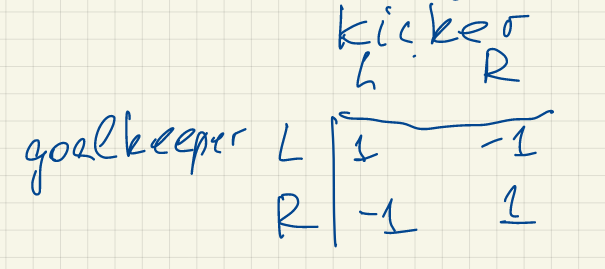
\includegraphics[scale=0.4]{penalty-game}
    \caption{penalty game}
  \end{figure}
\end{frame}

\begin{frame}
  \frametitle{Example: prisoners dilemma}
  \begin{figure}[ht]
    \centering
    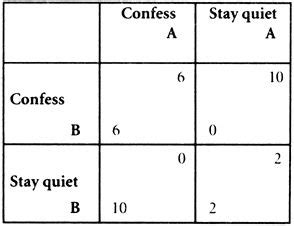
\includegraphics[width=0.5\textwidth]{prison}
    \caption{prisoners dilemma (not zero-sum)}
  \end{figure}
\end{frame}

\begin{frame}
  \frametitle{Worst case}

  \begin{itemize}
    \item if Alice chooses strategy $i$ she gets (at least): $\min_{j\in [n]} a_{i,j}$
    \item Alice can ensure payoff $\max_{i\in [m]} \min_{j\in [n]} a_{i,j}$
    \item Bob pays (at most) $\min_{j\in [n]} \max_{i\in [m]} a_{i,j}$
  \end{itemize}
  \onslide<2->{%
    We claim:
    \begin{equation}
      \max_i \min_j a_{i,j} \le \min_{j} \max_i a_{i,j}
    \end{equation}
    \begin{center}
      \textit{``Tallest dwarf is not as tall as the smallest giant.''}
    \end{center}
    But: \textbf{No equality in general!}
  }
\end{frame}

\begin{frame}
  \frametitle{Proof of the min-max theorem}
  \begin{equation}
    \begin{aligned}
      a_{ij} &\le a_{ij} & \forall i,j \\
      a_{ij} &\le \max_i a_{ij} & \forall i,j\\
      \min_j a_{ij} &\le \min_j \max_i a_{ij} & \forall i\\
    \end{aligned}
  \end{equation}
  \onslide<2->{%
  \begin{definition}
    We call $(i^*, j^*)$ a saddle point (or \emph{Nash equilibrium}) if
    \begin{equation}
      \max_i a_{ij^*} = a_{i^*j^*} = \min_j a_{i^*j}.
    \end{equation}
    These are called \emph{pure strategies}.
  \end{definition}
  }
\end{frame}

% Talk about stackelberg?

\begin{frame}
  \frametitle{Rock paper scissors}
  \begin{equation}
    \begin{array}{l|ccc}
        & R & P & S \\
      \hline
      R & 0 & -1 & 1 \\
      P & 1 & 0 & -1 \\
      S & -1 & 1 & 0
    \end{array}
  \end{equation}
  \begin{center}
    \textbf{No saddle-point!}
  \end{center}
  \vspace{1cm}
  \onslide<2->{%
    \center\textit{With pure strategies we do not always have a saddle point.}
  }

\end{frame}

\begin{frame}
  \frametitle{Mixed Strategies}
  \begin{block}{von Neumann (1928) --- Mixed strategies}
    \begin{itemize}
      \item Alice picks strategies $1, \dots, m$ \emph{with probabilities} $x\in \Delta_m$
      \item Bob picks strategies $1, \dots, n$ \emph{with probabilities} $y\in \Delta_n$
    \end{itemize}
    Expected gain of Alice is
    \begin{equation}
      \langle Ax, y \rangle = \sum_{i,j} a_{ij} x_i y_j
    \end{equation}
  \end{block}
  \onslide<2->{%
    \begin{theorem}[Saddle point exists]
      Expected gain of Alice $=$ expected loss of Bob
      \begin{equation}
        \max_{x \in \Delta} \min_{y \in \Delta} \langle Ax, y \rangle = \min_{y \in \Delta} \max_{x \in \Delta} \langle Ax, y \rangle.
      \end{equation}

    \end{theorem}
  }
\end{frame}

\section{Algorithms}%
\label{sec:}

\begin{frame}
  \frametitle{Stopping criteria}
  \begin{equation}
    \begin{aligned}
      \min_{x \in \Delta} \,\underbrace{\max_{y \in \Delta} \langle Ax, y \rangle}_{f_p(x)} =: \bm{v}  = \max_{y \in \Delta} \, \underbrace{\min_{x \in \Delta} \langle Ax, y \rangle}_{f_d(y)}
    \end{aligned}
  \end{equation}
  \begin{block}{stopping criterion}
    \begin{equation}
      \begin{aligned}
        f_p(x) - f_p(x^*) &= f_p(x) - v \onslide<2->{\textcolor{red}{\, \le \epsilon/2}}\\
        f_d(y^*) - f_d(y) &= v - f_d(y) \onslide<2->{\textcolor{red}{\, \le \epsilon/2}} \\
        \onslide<2->{\Rightarrow f_p(x) - f_d(y) \le \epsilon}
      \end{aligned}
    \end{equation}
  \end{block}
  \onslide<2->{%

  \begin{center}
    Before we never had the optimal value!
  \end{center}
  \textcolor{gray}{
  $f_p$ and $f_d$ is easy to compute (solution is on the boundary):
  \begin{equation}
    f_p(x) = \max_{y \in \Delta} \, \langle A x, y \rangle = \max_{j} \, \langle A x, e_j \rangle
  \end{equation}}
  }
\end{frame}


\begin{frame}
  \frametitle{}
  Consider
  \begin{equation}
      \min_{x \in \Delta}\,  \max_{y \in \Delta} \, \langle Ax, y \rangle
  \end{equation}
  as a minimization problem
  \begin{equation}
      \min_{x \in \Delta}\,   f_p(x) = \langle x, A^T y^* \rangle .
  \end{equation}
  Then, by the \textbf{first-order optimality condition}
  \begin{equation}
    x^* \in \argmin_{x \in \Delta}\,  f_p(x)  \Leftrightarrow \langle \nabla f_p(x^*), x-x^* \rangle \ge 0 \quad \forall x \in \Delta
  \end{equation}
  Thus
  \begin{equation}
    \begin{aligned}
      \langle A^T y^*, x-x^* \rangle &\ge 0 \quad \forall  x \in \Delta \\
      \langle -A x^*, y-y^* \rangle &\ge 0 \quad \forall  y \in \Delta \\
    \end{aligned}
  \end{equation}
  Concatenate the two conditions to get
  \begin{equation}
  \left\langle \begin{bmatrix}
      0 & A^T \\
      -A & 0
    \end{bmatrix}
    \left(\begin{array}{c}
      x^*\\ y^*
    \end{array}  \right),
    \left(\begin{array}{c}
      x \\ y
    \end{array}  \right)
    - % chktex 8
    \left(\begin{array}{c}
      x^* \\
      y^*
    \end{array} \right)
 \right\rangle \ge 0. % chktex 1
  \end{equation}
\end{frame}

\begin{frame}
  \frametitle{Games as Variational Inequalities}
  We had:
  \begin{equation}
  \left\langle \begin{bmatrix}
      0 & A^T \\
      -A & 0
    \end{bmatrix}
    \left(\begin{array}{c}
      x^*\\ y^*
    \end{array}  \right),
    \left(\begin{array}{c}
      x \\ y
    \end{array}  \right)
    - % chktex 8
    \left(\begin{array}{c}
      x^* \\
      y^*
    \end{array} \right)
 \right\rangle \ge 0. % chktex 1
  \end{equation}
  By rewriting $z=(x,y)$ and $F(z) = [A^T y; -Ax]$, then
  \begin{equation}\tag{VI}
    \label{eq:VI}
    \langle F(z^*), z-z^* \rangle \ge 0 \quad \forall z \in \Delta_n \times \Delta_m =: C
  \end{equation}
  \begin{center}
    \textbf{Variational inequality}
  \end{center}

  \begin{block}{}
  If $F = \nabla \phi$ then~\eqref{eq:VI} would be equivalent to
  \begin{equation}
    \min_{z\in C} \, \phi(z)
  \end{equation}
  \end{block}
\end{frame}

\begin{frame}
  \frametitle{Potential --- integrability}

  \textbf{Question:} Does there exist a potential $\phi$ for $F$, such that $F = \nabla \phi$

  \begin{block}{Integrability condition (from calculus)}
    Is the case if
    \begin{equation}
      \frac{\partial \phi}{\partial x \partial y} = \frac{\partial \phi}{\partial y \partial x}
    \end{equation}
  \end{block}
  But
  \begin{equation}
    \frac{\partial F_1}{\partial y} = \frac{\partial}{\partial y} A^T y = A^T \neq - A = \frac{\partial}{\partial x} -Ax =\frac{\partial F_2}{\partial x}.
  \end{equation}
  \textcolor{gray}{Recall
    \begin{equation}
      F = \begin{bmatrix}
      0 & A^T \\
      -A & 0
    \end{bmatrix}.
    \end{equation}}
\end{frame}


\begin{frame}
  \frametitle{VI as Fixed point equation}
  \begin{block}{}
    \vspace{-0.5cm}
  \begin{align}
    \langle F(z^*), z-z^* \rangle \ge 0 \quad \forall z \in C \\
    \Leftrightarrow z^* = P_C (z^* - F(z^*)) \label{eq:FP}\tag{FP}
  \end{align}
  \end{block}
  \begin{proof}
    Applying the property of the projection
    \begin{equation}
      \langle P_C(x)-x, x' - P_C(x) \rangle \ge 0 \quad \forall x' \in C
    \end{equation}
    with~\eqref{eq:FP}, gives
    \begin{equation}
    \langle z^* - (z^* - F(z^*)), z-z^* \rangle \ge 0 \quad \forall z \in C.\hfill \qedhere\qed
    \end{equation}
  \end{proof}
  \begin{itemize}
    \item should remind us of (projected) gradient descent
          \item when you see a \textbf{\textcolor{blue}{fixed point equation: iterate!}}
  \end{itemize}
\end{frame}


\begin{frame}
  \frametitle{But is it any good?}
  Consider the \textbf{unconstrained case}
  \begin{equation}
    \langle F(z^*), z-z^* \rangle \ge 0 , \, \forall z  \quad \Leftrightarrow \quad F(z^*) = 0.
  \end{equation}
  \begin{equation}
    z_{k+1} = z_k - \alpha F(z_k)
  \end{equation}
  Then
  \begin{equation}
    \begin{aligned}
      \Vert z_{k+1} \Vert^2 &= \Vert z_k \Vert^2 - \underbrace{2 \alpha \langle F(z_k), z_k \rangle}_{=0} + \alpha^2 \Vert F(z_k) \Vert^2 \\
      &=\Vert z_k \Vert^2 + \alpha^2 \Vert F(z_k) \Vert^2 \\
    \end{aligned}
  \end{equation}
  Resulting in $\Vert z_{k+1} \Vert \ge \Vert z_k \Vert$.
  \begin{center}
    $\Rightarrow$ \textbf{No bueno!}
  \end{center}
\end{frame}


\begin{frame}
  \frametitle{}

We can still show
  \begin{theorem}
    Convergence rate for \textbf{averaged iterates} in terms of \textbf{primal-dual gap}
    \begin{equation}
      f_p(\bar{x}_k) - f_d(\bar{y}_k) \le \frac{C}{ \sqrt{k}},
    \end{equation}
    where $\bar{x}_k = \frac{1}{k} \sum_{i=0}^{k-1} x_i $
  \end{theorem}

  \begin{itemize}
    \item with the same analysis as for subgradient descent
  \end{itemize}
\end{frame}

\begin{frame}
  \frametitle{Sketch of the proof}
  With the notation $g_k = F(z_k)$ we get
  \begin{equation}
    \begin{aligned}
      \Vert x_{k+1} - x^* \Vert^2 &\le \Vert x_k - \alpha_k g_k - x^* \Vert^2 \\
      &= \Vert x_k-x^* \Vert^2 + 2 \alpha_k \langle g_k, x^*-x_k \rangle + \alpha^2 \Vert g_k \Vert^2.
    \end{aligned}
  \end{equation}
  But this time $\langle g_k, x^* - x_k \rangle = [f_d(y_k) - f_p(x_k)]$.
  % Rest of the proof is left as an exercise.
\end{frame}


\begin{frame}
  \frametitle{A better method}

  \begin{algorithm}[H]
    \caption{Extragradient Method [1976]}
    \begin{algorithmic}[1]
      \For{$k = 1,2, \dots$}
      \State{ $w_{k+1} = z_k  - \alpha_k F(z_k)$}
      \State{ $z_{k+1} = z_k  - \alpha_k F(w_k)$}
      \EndFor{}
    \end{algorithmic}
  \end{algorithm}

  \begin{itemize}
    \item more conservative
    \item works for general min-max problems
          \begin{equation}
            \min_x \max_y \, \Phi(x,y) \quad \Rightarrow F(x,y) = {(\nabla_x \Phi(x,y), - \nabla_y \Phi(x,y))}^T
          \end{equation}
    \item can even improve behavior of pure minimization ($F = \nabla f$)
    \item improved rate of $\mathcal{O}(1/k)$ for averaged iterates
  \end{itemize}
\end{frame}

\section{More min-max problems}%
\label{sec:}

\begin{frame}
  \frametitle{Robust Optimization}
  \begin{itemize}
    \item uncertainty in the \textbf{objective} ($u \in U$ \text{ \textcolor{blue}{uncertainty set}})
          \begin{equation}
            \min_x f(x, u)
          \end{equation}
    \item bound the \textbf{worst case}
          \begin{equation}
            \min_x \max_{u \in U}\, f(x, u)
          \end{equation}
  \end{itemize}
\end{frame}

\begin{frame}
  \frametitle{Vulnerability of Neural Networks}
  \begin{minipage}{0.45\textwidth}
    \begin{figure}[ht]
      \centering
      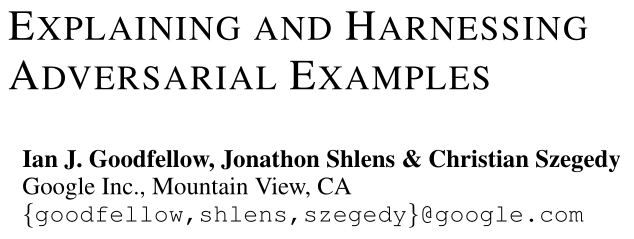
\includegraphics[width=\textwidth,keepaspectratio]{vulnerable3}
      % \caption{\label{fig:label} }
    \end{figure}
  \end{minipage}
  \begin{minipage}{0.5\textwidth}
    \begin{figure}[ht]
      \centering
      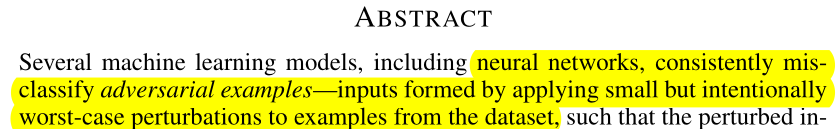
\includegraphics[width=\textwidth,keepaspectratio]{vulnerable4}
    \end{figure}
  \end{minipage}

  \begin{figure}[ht]
    \centering
    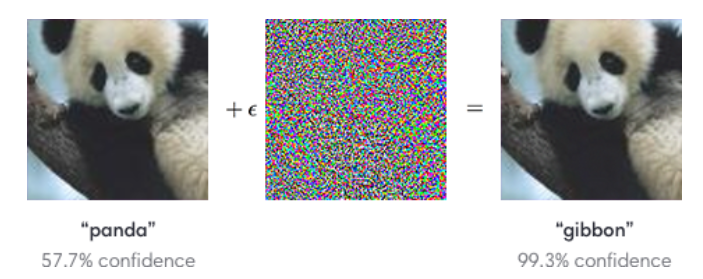
\includegraphics[width=\textwidth,height=\textheight,keepaspectratio]{adversarial-example}
    \caption{$\epsilon=0.007$}
  \end{figure}
\end{frame}


\begin{frame}
  \frametitle{Vulnerability in ``real life''}
  \begin{figure}[ht]
    \centering
    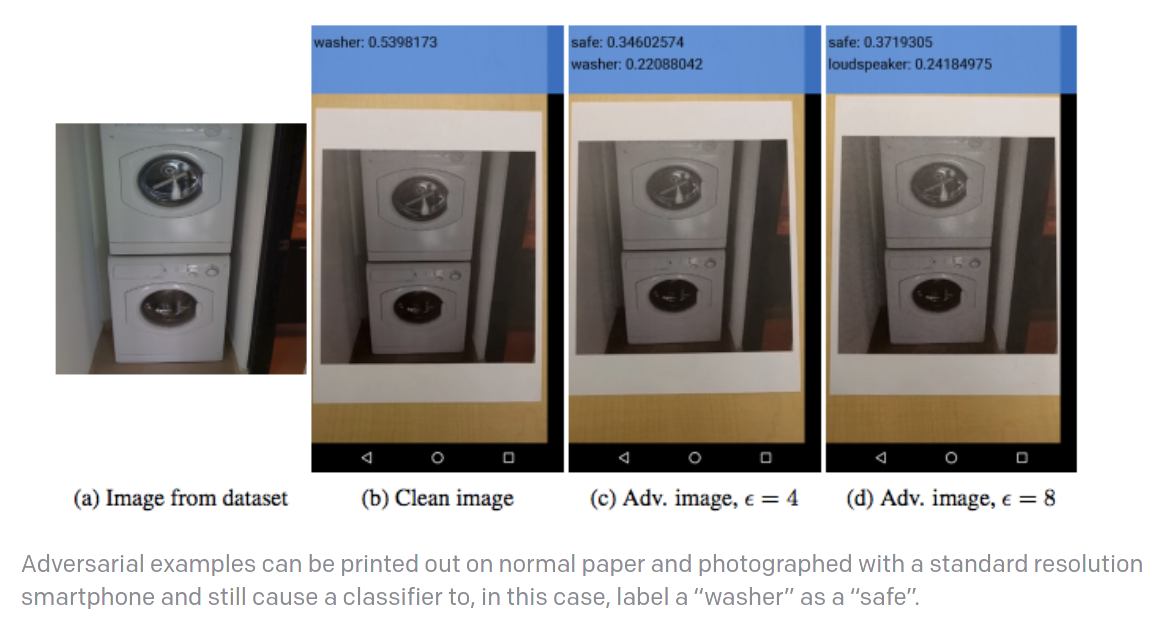
\includegraphics[width=\textwidth,height=\textheight,keepaspectratio]{washer}
  \end{figure}
\end{frame}


\begin{frame}
  \frametitle{Generation of adversarial examples}
  \begin{block}{Training objective}
    \begin{equation}
      \min_\theta J(\theta, x, y)
    \end{equation}
    \begin{itemize}
      \item $\theta$ parameters (weights, biases)
      \item $x$ images
      \item $y$ corresponding labels
    \end{itemize}
  \end{block}
  \begin{block}{Attack direction (``white box'')}
    \begin{equation}
      \nabla_x J(\theta, x, y)
    \end{equation}
  \end{block}
  Typically only the sign is used.
\end{frame}

\begin{frame}
  \frametitle{Adversarial training}

  \begin{block}{Augment training data with adversarial examples}
    \begin{itemize}
      \item grab a fresh training example $x$
      \item perturb image: $\tilde{x} \leftarrow x - \epsilon \text{sign}(\nabla_x J(\theta, x, y))$
      \item update weights:  $\theta \leftarrow \theta - \nabla_\theta J(\theta, \tilde{x}, y)$
    \end{itemize}
  \end{block}

  Corresponds to solving the robust \textcolor{blue}{min-max} problem
  \begin{align}
    &\min_\theta \max_{\tilde{x}} \, J(\theta, \tilde{x}, y) \\
    &\text{s.t. } \Vert \tilde{x}-x \Vert_\infty \le \epsilon
  \end{align}
\end{frame}


\begin{frame}
  \frametitle{GANs}
  \begin{figure}[ht]
    \centering
    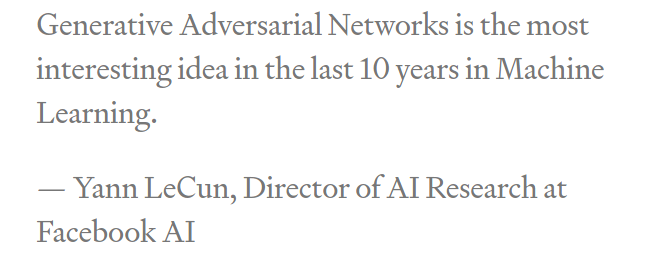
\includegraphics[width=\textwidth]{GAN_quote.png}
    % \caption{\label{fig:label} }
  \end{figure}
\end{frame}


\begin{frame}
  \frametitle{What do they \emph{generate}?}
    \begin{figure}[ht]
      \centering
      \begin{subfigure}[c]{.45\textwidth}
        
\includegraphics[width=\linewidth]{one_does_not_simply.jpg}
      \end{subfigure}
      \begin{subfigure}[c]{.52\textwidth}
        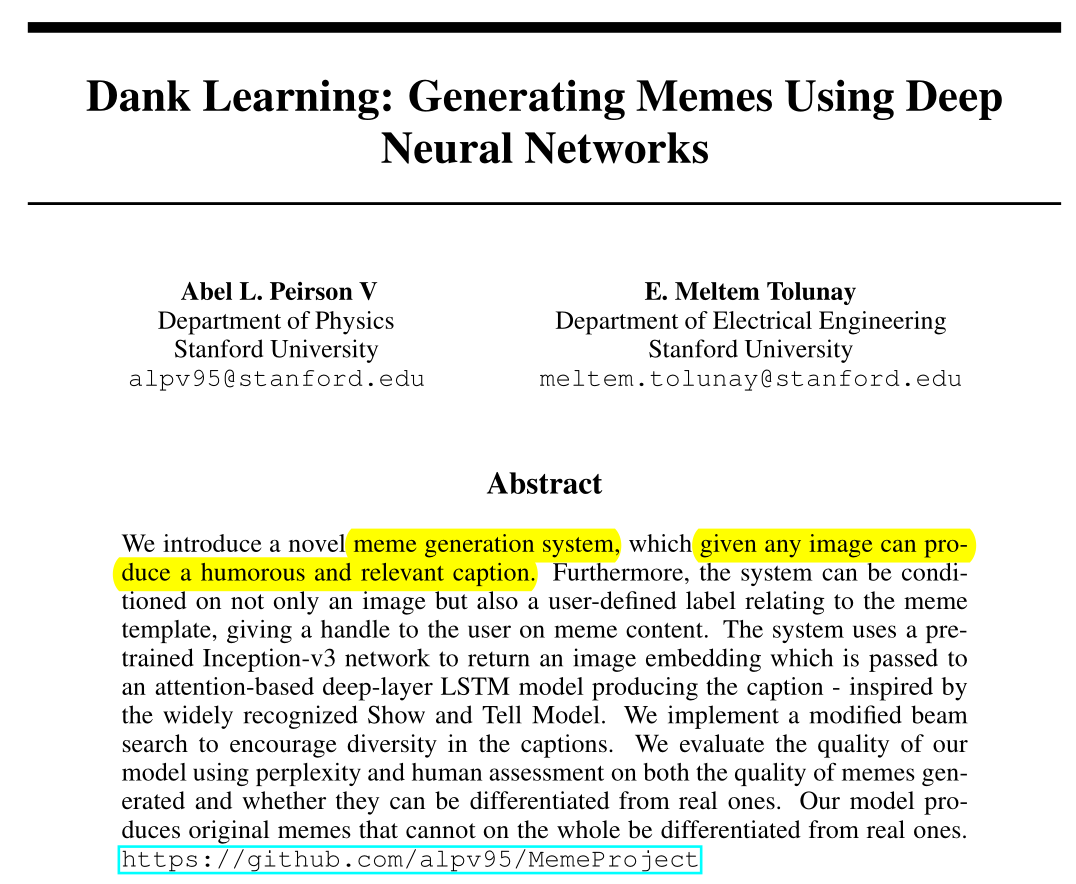
\includegraphics[width=\linewidth]{paper_generating_memes.png}
      \end{subfigure}
    \end{figure}
\end{frame}



\begin{frame}
  \frametitle{How did they do?}
  \begin{figure}[ht]
    \centering
    
\includegraphics[width=\textwidth]{generated_memes.jpg}
  \end{figure}
\end{frame}


\begin{frame}
  \frametitle{More serious applications (inpainting)}
  \begin{figure}[ht]
    \centering
    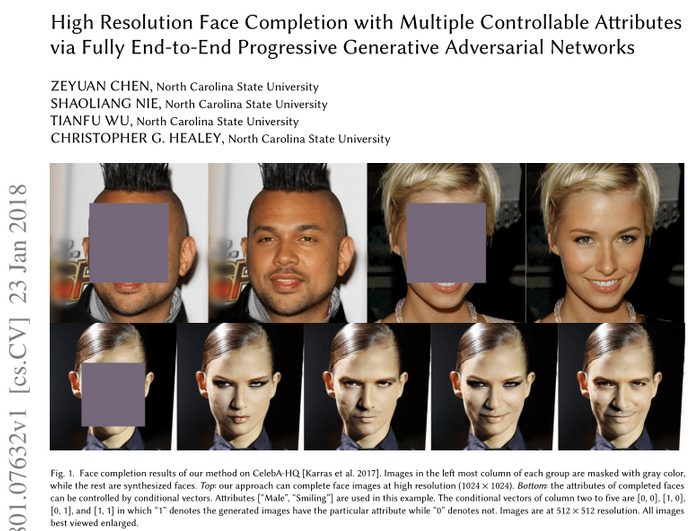
\includegraphics[scale=0.4]{inpainting}
    % \caption{\label{fig:label} }
  \end{figure}
\end{frame}


\begin{frame}
  \frametitle{Or less serious\ldots}

    \begin{figure}[ht]
      \centering
      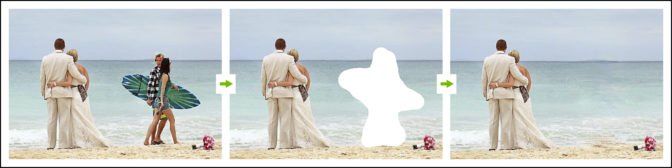
\includegraphics[width=\textwidth]{inpainting_beach}
      % \caption{\label{fig:label} }
    \end{figure}
\end{frame}

\begin{frame}
  \frametitle{Creating Art}

    \begin{figure}[ht]
      \centering
      \begin{subfigure}[c]{.47\textwidth}
        
\includegraphics[width=\linewidth]{GAN_price}
      \end{subfigure}
      \begin{subfigure}[c]{.47\textwidth}
        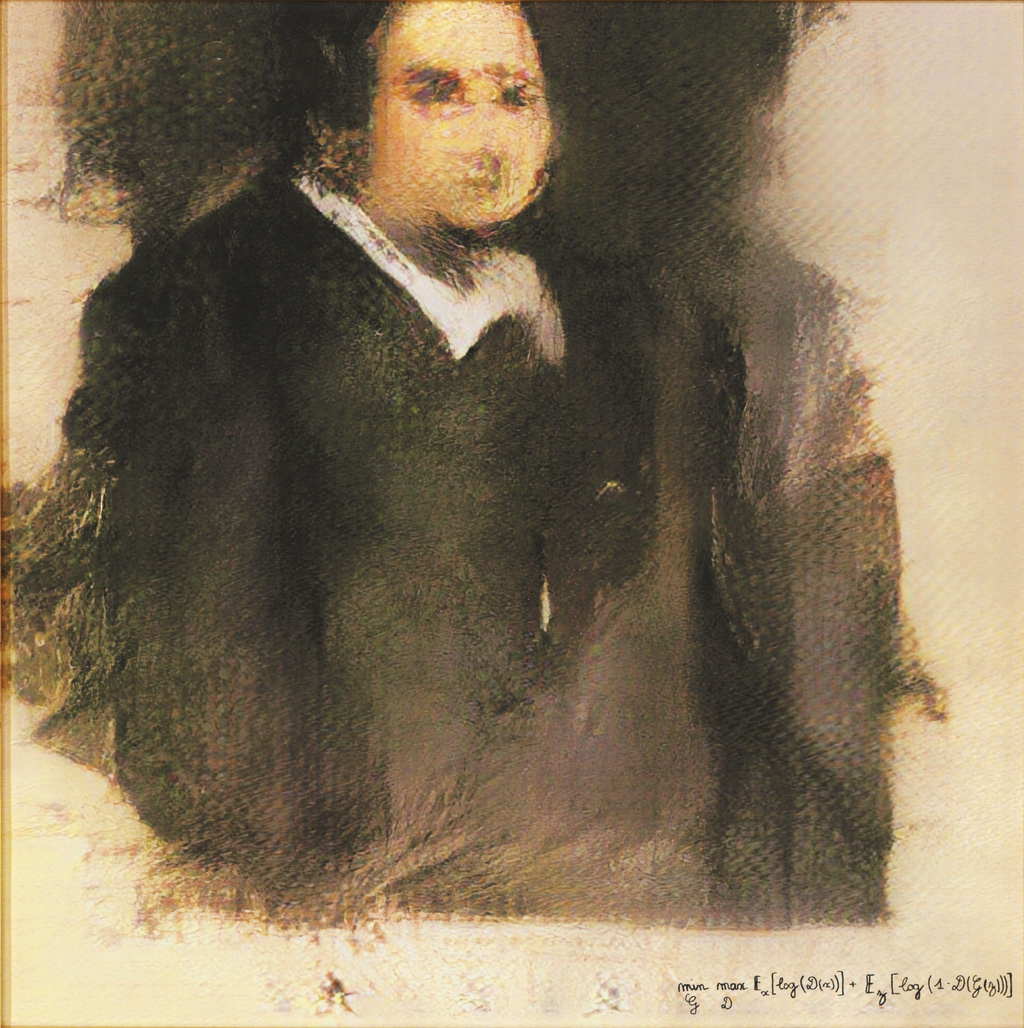
\includegraphics[width=\linewidth]{expensive_GAN}
      \end{subfigure}
    \end{figure}
\end{frame}


\begin{frame}
  \frametitle{Why Adversarial?}
  Two NNs trained at the same time.
  \begin{figure}[ht]
    \centering
    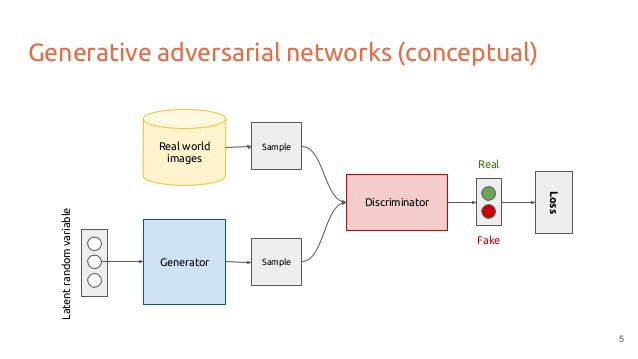
\includegraphics[width=.95\textwidth]{GAN}
    % \caption{\label{fig:label} }
  \end{figure}
\end{frame}


\begin{frame}
  \frametitle{GANs mathematically}
  Given by the \textcolor{blue}{\emph{two-player game}}.
  \begin{equation}
    \min_{\G} \max_{\D} \, \E_{x\sim p_{data}} [\log(\D(x))] + \E_{z\sim p_{noise}}
    [\log(1- \D(\G(z)))]
  \end{equation}
  where
  \begin{itemize}
    \item $p_{z}(z)$ is the input noise variable,
    \item $\G$ is the \emph{generator},
    \item $\D$ is the \emph{discriminator}.
  \end{itemize}
  \begin{block}{}
    Discriminator gives probability that $x$ came from the (true) data rather than
    from the generator.
  \end{block}
\end{frame}



\end{document}
